\documentclass[conference]{IEEEtran}
\IEEEoverridecommandlockouts

\usepackage[utf8]{inputenc}
\usepackage[T1]{fontenc}
\usepackage{cite}
\usepackage{amsmath,amssymb,amsfonts}
\usepackage{graphicx}
\usepackage{textcomp}
\usepackage{xcolor}
\usepackage{url}
\usepackage{booktabs}
\usepackage{tikz}
\usetikzlibrary{positioning,arrows.meta,fit,backgrounds,calc}

\def\BibTeX{{\rm B\kern-.05em{\sc i\kern-.025em b}\kern-.08em
    T\kern-.1667em\lower.7ex\hbox{E}\kern-.125emX}}

\begin{document}

\title{Concurrency-Aware SLA Scheduling and Admission Control for Analytical Queries in a Data Lake}

\author{
\IEEEauthorblockN{Rupali Guleria}
\IEEEauthorblockA{
% TODO(Rupali): confirm affiliation line before arXiv upload -- email is set, affiliation below is still a default guess.
Independent Researcher\\
Email: guleriarupali27@gmail.com}
}

\maketitle

\begin{abstract}
Lakehouse query engines increasingly serve mixed analytical workloads under per-query deadlines alongside continuous ingestion, commonly assumed the primary risk to deadline compliance. Four independent tests show otherwise: ingestion has little measurable effect on query latency here; query concurrency is the dominant factor -- a single-node Trino deployment slows a point-lookup query 19$\times$ at sixteen concurrent queries versus one. We reframe scheduling accordingly. Conditioning runtime prediction on current concurrency materially changes scheduling decisions in simulation, and live evaluation confirms the broader contention-driven collapse in deadline adherence and the aggregate advantage of dynamic-programming (DP) based scheduling, though not a consistent live edge for adaptive over static prediction specifically. An objective-optimal DP scheduler closes much of the remaining gap. Beyond a certain concurrency level no ordering satisfies every deadline; the more defensible response is admission control, deferring excess load rather than letting it fail: admitted queries met deadlines more often than the blended average in every live condition tested, and under live moderate-concurrency contention the mechanism deferred 82.5\% of arrivals once its feasibility test judged further admission unsafe. We report ingestion's null effect as a rigorously tested finding, and state this work's scope plainly: predictions are point estimates, concurrency is modeled at three coarse levels, and one live admission-control result falls short of its predicted target -- discussed, not hidden.
\end{abstract}

\begin{IEEEkeywords}
lakehouse systems, query scheduling, admission control, query concurrency, SLA-aware systems, Trino
\end{IEEEkeywords}

\IEEEpeerreviewmaketitle

\section{Introduction}

Query engines that serve interactive dashboards alongside heavier analytical workloads must decide, at any given moment, which of several waiting queries to execute next. An uninformed ordering decision can leave a small, urgent dashboard query queued behind a large report with no compensating benefit. This problem is sharper in a lakehouse architecture, where the query engine and the storage layer are separate systems connected over a network, and where the same compute cluster is frequently shared between reading data (queries) and writing it (ingestion).

This work is motivated by a specific question: does ingestion activity degrade query latency enough that a scheduler should explicitly account for it? If so, a scheduler that detects heavy ingestion could predict slower query execution and adjust its ordering accordingly. This is, on its face, a reasonable expectation -- ingestion and queries can compete for the same disks, network bandwidth, and compute -- and it was the premise underlying the initial design of this project.

This hypothesis did not hold at the scale evaluated here. The dominant factor was instead one the initial design did not account for: the number of queries executing concurrently. This paper reports both findings -- the refutation of the ingestion hypothesis and the concurrency-aware scheduling and admission-control design that replaced it -- together with an evaluation spanning simulation, held-out validation, and live execution against a real Trino deployment.

The contributions of this paper are:

\begin{enumerate}
\item Four independent tests demonstrating that ingestion has negligible effect on query latency in this setting (Section~\ref{sec:ingestion}), motivating its exclusion as the primary scheduling signal.
\item A concurrency-aware scheduler design -- an adaptive least-slack heuristic and an exact dynamic-programming (DP) scheduler -- validated in simulation, against held-out data collected independently of calibration, and live against Trino (Sections~\ref{sec:problem} and~\ref{sec:results}).
\item An admission-control mechanism that detects when predicted system load exceeds what can be reliably served and defers rather than over-promises, with its core behavior -- admitted queries meeting deadlines more often than the blended average -- confirmed under live execution rather than simulation alone (Section~\ref{sec:admission}).
\end{enumerate}

\section{Background and Motivation}
\label{sec:background}

A lakehouse separates compute (the query engine, e.g., Trino) from storage (an object store, e.g., MinIO, accessed through a table format). Multiple queries, and frequently ingestion jobs, share the same compute cluster. Each arriving query is assigned a deadline determined by its SLA tier, and the system must decide, among all queries currently waiting, which to execute next.

A naive scheduler ignores system state entirely, ordering queries by arrival (FIFO), by priority alone, or by deadline alone. A slack-based scheduler is more deliberate: it computes each query's \emph{slack} -- the time remaining before its deadline minus its predicted runtime -- and executes the query with the least slack first. The accuracy of this approach depends entirely on the accuracy of the runtime prediction it is built on: if the system is under real contention but the prediction assumes an idle system, the resulting schedule can be substantially wrong.

The central design question this project addresses is what that prediction should be conditioned on. The initial hypothesis was ingestion load; Section~\ref{sec:ingestion} reports why this hypothesis was rejected and what replaced it.

\section{Problem Statement and Scheduler Designs}
\label{sec:problem}

We consider a batch of $n$ queries arriving simultaneously, each characterized by:

\begin{itemize}
\item a \textbf{query class} (short, medium, or long), reflecting the inherent cost of the query;
\item an \textbf{SLA tier} (relaxed, moderate, or tight), reflecting how much slack its deadline allows; and
\item a \textbf{priority} (1, highest, to 3, lowest) -- an independent measure of business importance, not derived from class or tier.
\end{itemize}

The system executes one query at a time (strictly serial execution; see Section~\ref{sec:limitations} for the rationale behind this scope) and must determine the order. We compare five schedulers, each isolating a single design variable, summarized in Table~\ref{tab:schedulers}.

\begin{table*}[t]
\caption{Schedulers compared in this paper. Each isolates a single design variable.}
\label{tab:schedulers}
\centering
\begin{tabular}{@{}p{0.16\textwidth}p{0.78\textwidth}@{}}
\toprule
\textbf{Scheduler} & \textbf{Rule} \\
\midrule
Static Least Slack & Always predicts runtime using the \emph{uncontended} baseline -- as if the system were always idle. \\[2pt]
Adaptive Least Slack & Predicts runtime using the \emph{current} concurrency level (low / moderate / high). Same ordering rule as Static -- the only difference is what it assumes about system load. \\[2pt]
DP Oracle & Given the same concurrency-aware predictions as Adaptive, computes the order that maximizes total priority-weighted predicted SLA success -- using priority weights $\{1{:}\,3,\ 2{:}\,2,\ 3{:}\,1\}$ (checked for robustness in Section~\ref{sec:robustness}) -- via dynamic programming over subsets of the batch, rather than a greedy rule. Optimal under those predicted runtimes and that objective, not a guarantee about what would actually happen if the predictions were wrong. Quantifies the room a smarter algorithm has to improve on the greedy heuristic. \\[2pt]
Admission-Controlled DP & Wraps the DP Oracle with a gate: before admitting each arriving query, it checks whether the \emph{predicted} success rate of everything admitted so far still meets a declared target (default 80\%). If not, the query is deferred, not dropped -- it still runs, just last, and is still scored against its original deadline. \\[2pt]
FIFO, Priority-First, EDF (reference only) & Naive baselines with no runtime-awareness at all, used to confirm that slack-based ordering is worth having in the first place. \\
\bottomrule
\end{tabular}
\end{table*}

The comparison between Static and Adaptive Least Slack isolates whether load-aware prediction materially changes scheduling decisions: the two share the same algorithm, tie-break rules, deadlines, and priorities, differing only in whether the runtime prediction reacts to current system load. The DP and admission-control experiments address a separate question -- how much further improvement is achievable through global ordering and feasibility-aware admission on top of that. These are distinct questions: this paper's central claim concerns schedulability under contention, not the margin by which one adaptive heuristic outperforms another, so a small Static-versus-Adaptive gap does not by itself undermine the DP or admission-control results.

\section{Experimental Setup}
\label{sec:setup}

\begin{figure}[t]
\centering
\resizebox{\columnwidth}{!}{%
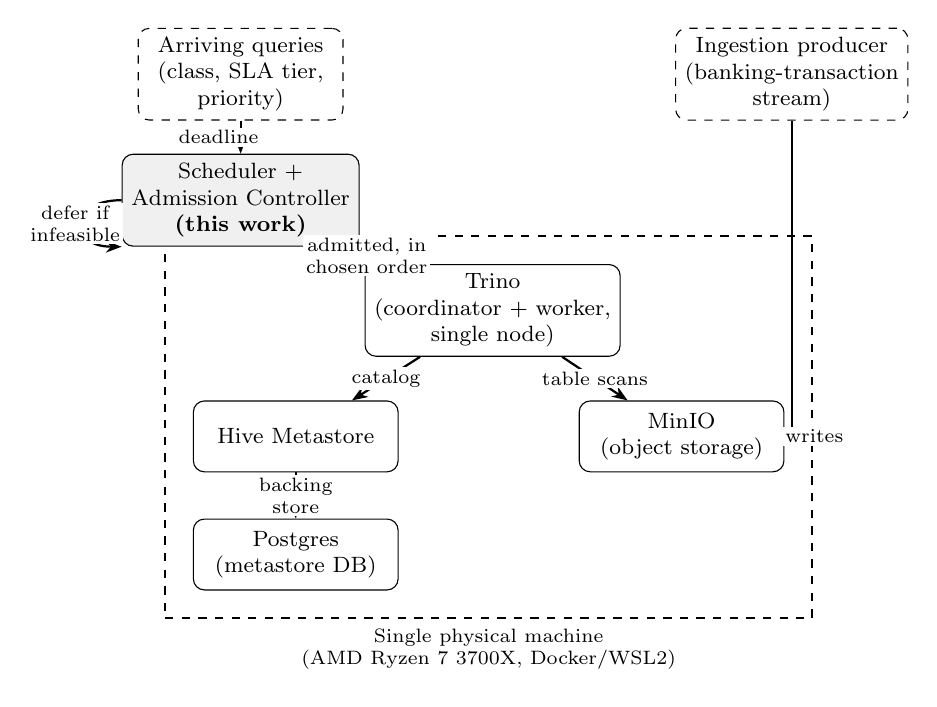
\begin{tikzpicture}[
  box/.style={draw, rectangle, rounded corners, align=center, minimum height=0.9cm, minimum width=2.6cm, font=\footnotesize},
  ext/.style={box, dashed},
  lbl/.style={font=\scriptsize, midway, align=center, fill=white, inner sep=1pt},
  arr/.style={-{Stealth[length=2mm]}, thick}
]

% External actors
\node[ext] (queries) at (0,4.6) {Arriving queries\\(class, SLA tier,\\priority)};
\node[ext] (ingest)  at (7,4.6) {Ingestion producer\\(banking-transaction\\stream)};

% Scheduling layer (this work)
\node[box, fill=gray!12] (sched) at (0,3.0) {Scheduler +\\Admission Controller\\\textbf{(this work)}};

% Inner machine components
\node[box] (trino) at (3.2,1.6) {Trino\\(coordinator + worker,\\single node)};
\node[box] (hive)  at (0.7,0.0) {Hive Metastore};
\node[box] (pg)    at (0.7,-1.5) {Postgres\\(metastore DB)};
\node[box] (minio) at (5.6,0.0) {MinIO\\(object storage)};

% Bounding box for the single physical machine
\begin{scope}[on background layer]
\node[draw, dashed, thick, inner sep=10pt, fit=(trino)(hive)(pg)(minio),
      label={[font=\scriptsize,align=center]below:Single physical machine\\(AMD Ryzen 7 3700X, Docker/WSL2)}] (machine) {};
\end{scope}

% Arrows
\draw[arr] (queries) -- (sched) node[lbl, pos=0.5, xshift=-8pt] {deadline};
\draw[arr] (sched) -- (trino) node[lbl] {admitted, in\\chosen order};
\draw[arr] (sched.west) to[out=180,in=180,looseness=3] node[lbl, xshift=-2pt] {defer if\\infeasible} (sched.south west);
\draw[arr] (ingest) |- (minio) node[lbl, pos=0.85, xshift=10pt] {writes};
\draw[arr] (trino) -- (hive) node[lbl] {catalog};
\draw[arr] (hive) -- (pg) node[lbl] {backing\\store};
\draw[arr] (trino) -- (minio) node[lbl] {table scans};

\end{tikzpicture}%
}
\caption{System architecture. Arriving queries pass through the scheduler and admission-control layer evaluated in this paper before reaching Trino; ingestion is a separate producer writing directly into object storage. All four backend services run as Docker containers on a single physical machine (Section~\ref{sec:setup}), which is the deployment constraint underlying the concurrency results in Section~\ref{sec:results}.}
\label{fig:architecture}
\end{figure}

\textbf{Hardware.} All experiments run on a single physical machine, shown in Fig.~\ref{fig:architecture}: an AMD Ryzen~7 3700X (8 cores / 16 threads) with 32\,GB RAM and over 300\,GB of free SSD storage, running Windows with Docker Desktop under WSL2. This machine hosts Trino, MinIO (object storage), a Hive metastore, and Postgres, all via Docker. WSL2/Docker is configured with 24\,GB RAM and 12 of the 16 physical threads (\texttt{infra/.wslconfig}), and Trino itself runs with a 16\,GB heap (\texttt{-Xmx16G}) within that allocation -- Trino therefore never has access to the full physical machine, a constraint relevant to interpreting the concurrency results in Section~\ref{sec:results}. A query against \texttt{system.runtime.nodes} confirms that exactly one node acts as both coordinator and worker, i.e., this is a single-node deployment rather than a cluster, which is likewise relevant to interpreting the concurrency results.

\textbf{Data.} Experiments use TPC-H at scale factor 0.1 (600{,}572 \texttt{lineitem} rows, 150{,}000 \texttt{orders} rows), queried through three classes: \texttt{short} (a point lookup), \texttt{medium} (an aggregation), and \texttt{long} (a join). Ingestion traffic is generated from a separate synthetic banking-transaction stream, deliberately distinct from the queried tables, so that ingestion volume can be varied independently of query data size.

\textbf{Evaluation.} We report results from three evaluation layers rather than selecting one:

\begin{enumerate}
\item \emph{Bootstrap simulation} -- 1{,}000 synthetic batches (4--10 queries each), constructed by resampling real per-query timing measurements. This is the fastest evaluation layer, but because the same measurement pool is used both to build the prediction and to score against it, it is the weakest test of generalization.
\item \emph{Held-out evaluation} -- the identical 1{,}000 batches, scored against a second, independently collected round of timing measurements (collected on a different day) rather than the calibration pool. This isolates whether results are an artifact of testing on the same data used to fit the predictor.
\item \emph{Live evaluation} -- schedulers' decisions are executed against the live Trino deployment: each query in a batch is run in the order the scheduler selects and scored against its measured runtime. This is the strongest evaluation, since nothing is simulated, but it has the smallest sample size (dozens to low hundreds of queries per condition, versus thousands in simulation) and is the most sensitive to environmental noise (Section~\ref{sec:limitations}).
\end{enumerate}

\textbf{Reproducibility control.} Live testing on a continuously running, single-machine deployment proved sensitive to the machine's own state (Section~\ref{sec:limitations}). We therefore verify, before every live session, that uncontended query latency matches the calibration baseline, and abort the session if it has drifted by more than 50\% (\texttt{scripts/ryzen\_health\_check.py}). This check is a methodological safeguard for reproducibility; it is not evidence for any of the paper's substantive claims.

\section{Ingestion Contention Is Not the Dominant Scheduling Signal}
\label{sec:ingestion}

The initial scheduler design conditioned runtime prediction on \texttt{ingestion\_condition} (none, moderate, or heavy sustained ingestion). Four independent tests, conducted at different stages of the project using different methods, converge on the same conclusion:

\begin{enumerate}
\item \textbf{Single-query timing.} Running individual queries under each ingestion condition produced runtime shifts of only 2--21\,ms -- within measurement noise, relative to the hundreds to thousands of milliseconds of actual slack between queries in a typical batch.
\item \textbf{1{,}000-batch simulation.} Because the ingestion signal barely affected the prediction, Static and Adaptive Least Slack produced identical execution orders across all 1{,}000 simulated batches (0/1000 differed): an ingestion-conditioned scheduler had, in practice, nothing to adapt to.
\item \textbf{Live multi-query validation.} Real batches executed against Trino under none/moderate/heavy ingestion conditions showed flat SLA adherence across all three conditions -- no scheduler's live success rate moved meaningfully with ingestion load.
\item \textbf{Corrected re-test.} A subsequent investigation identified a data-registration defect: ingested data was never actually registered in Trino's table catalog, so ``ingestion'' was invisible to every query throughout the earlier tests. After correcting this (properly syncing ingested data and maintaining a continuously streaming producer) and repeating the comparison, no scheduler's adherence differed by more than approximately 4 percentage points between the no-ingestion and ingestion-visible conditions.
\end{enumerate}

At the scale and architecture evaluated here, ingestion-induced contention has little measurable effect on steady-state analytical query latency. We report this as a substantive negative result rather than an implementation failure: it was tested four independent ways and never contradicted, and it motivates the concurrency-centered design used throughout the remainder of this paper.

One observation merits note for future work: the \texttt{long} (join) query class exhibited a heavier tail under visible ingestion (mean 3.7$\times$ the median), plausibly because an actively growing partition is occasionally scanned mid-write. The corresponding sample (464 queries) is too small to support a claim on this point.

\section{Results}
\label{sec:results}

\subsection{Concurrency Is the Dominant Driver}

Testing concurrent query execution in isolation (no ingestion) produced a markedly different result: increasing load from one query at a time to sixteen concurrent queries slowed the same point-lookup query by a factor of 19 (mean 296\,ms to 5{,}717\,ms across the calibration rounds at each level), consistent with the single-node deployment described in Section~\ref{sec:setup} -- every concurrent query competes for the same limited execution slots, since no second node is available to distribute the load. Fig.~\ref{fig:concurrency-runtime} shows this effect across the full concurrency sweep and all three query classes.

\begin{figure}[t]
\centering
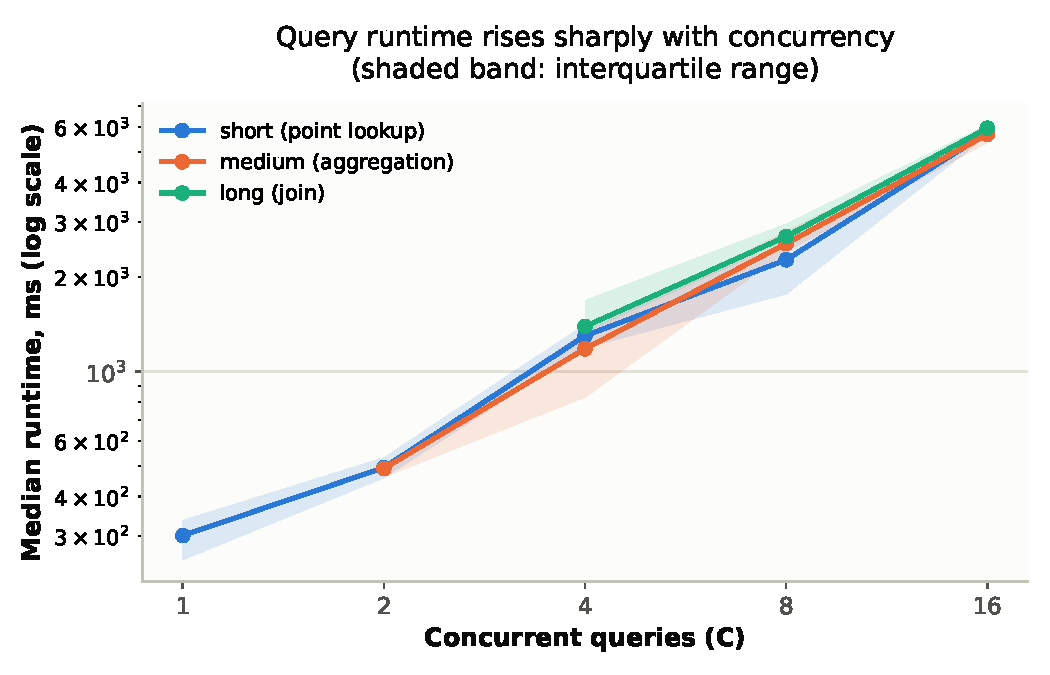
\includegraphics[width=\columnwidth]{figures/fig_concurrency_runtime.pdf}
\caption{Median runtime versus concurrent query count, by query class, from the calibration sweep (\texttt{results/week4/concurrency\_contention.csv}; shaded band: interquartile range). Lines are plotted from per-cell \emph{medians}, the same statistic the Adaptive scheduler's predictions use (Section~\ref{sec:background}); this differs slightly from the \emph{mean}-based single-query figure quoted in the text above, which both indicate the same $\sim$19$\times$ effect. Sample sizes are small at low concurrency ($n{=}4$ per cell in several cases) and uneven across classes -- the sweep only cycles the \texttt{short} class at $C{=}1$, so the \texttt{medium} and \texttt{long} lines begin at $C{=}2$ and $C{=}4$ respectively.}
\label{fig:concurrency-runtime}
\end{figure}

When the Adaptive scheduler's prediction was reconditioned on concurrency level rather than ingestion condition, Static and Adaptive Least Slack's chosen execution order diverged in 488 of 1{,}000 simulated batches, compared to 0 of 1{,}000 under the ingestion-based signal. Concurrency shifts predicted runtime by hundreds to thousands of milliseconds -- comparable to the actual slack spread between queries in a batch -- which is precisely the condition under which an adaptive predictor has anything to contribute.

\subsection{Offline Scheduler Comparison}

\begin{figure}[t]
\centering
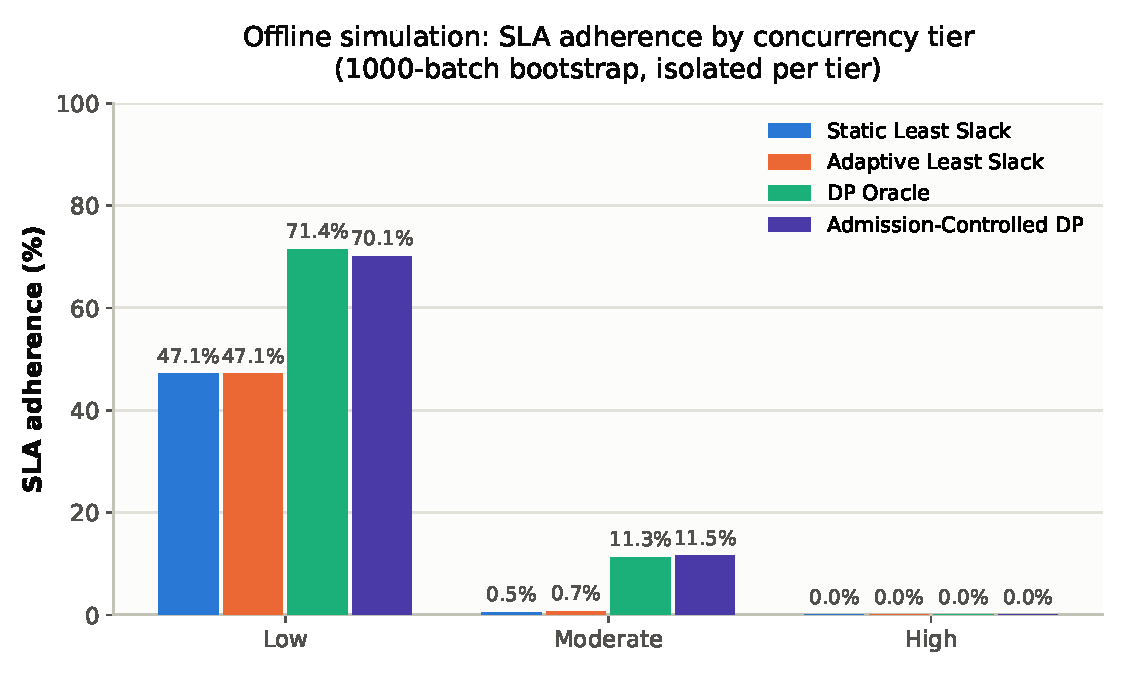
\includegraphics[width=\columnwidth]{figures/fig1_offline_per_tier.pdf}
\caption{SLA adherence by scheduler, isolated per concurrency tier (1{,}000-batch bootstrap simulation).}
\label{fig:offline-per-tier}
\end{figure}

At \textbf{low} concurrency, every scheduler achieves reasonable adherence (47--71\%), with the DP-based schedulers (DP Oracle, Admission-Controlled DP) leading (Fig.~\ref{fig:offline-per-tier}). At \textbf{moderate} concurrency, adherence collapses by an order of magnitude or more across all schedulers (0.5--11.5\%), indicating that moderate concurrency already approaches this hardware's effective ceiling. At \textbf{high} concurrency, every scheduler -- including the DP Oracle, which is optimal under the predicted runtimes and the chosen objective -- reaches \textbf{0\%} adherence. This is not attributable to any particular algorithm: deadlines were set relative to uncontended performance, and at high concurrency the workload becomes genuinely infeasible to complete on time regardless of ordering. This is precisely the condition admission control (Section~\ref{sec:admission}) is designed to detect and respond to, rather than silently fail against.

\subsection{Live Evaluation}

\begin{figure}[t]
\centering
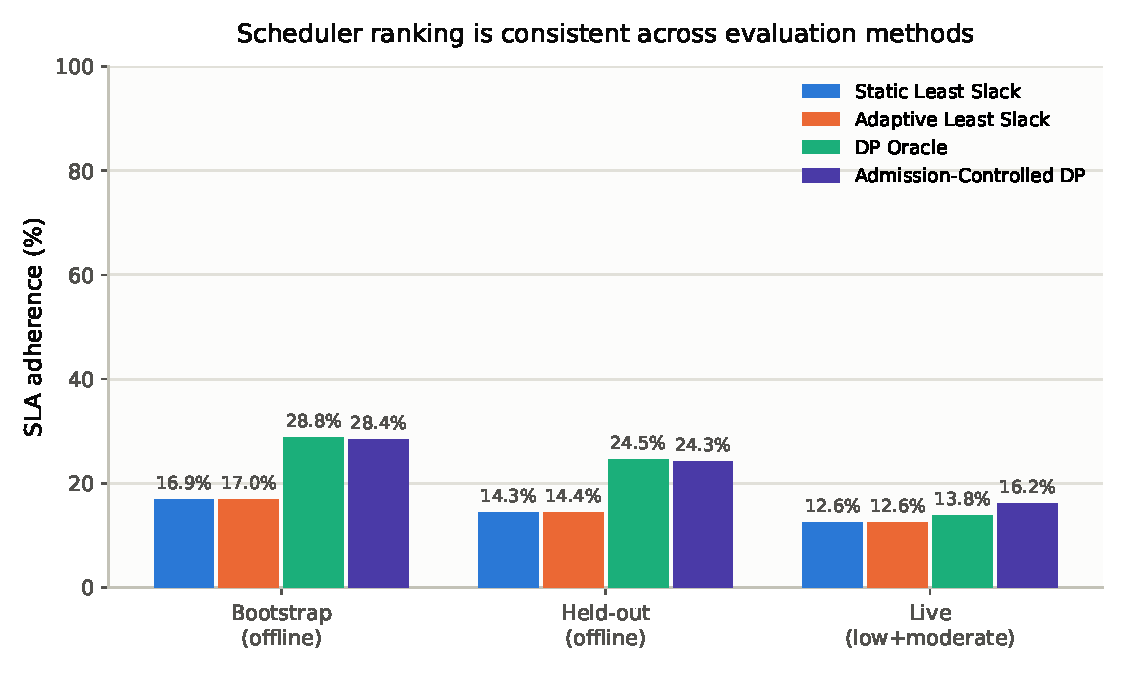
\includegraphics[width=\columnwidth]{figures/fig2_offline_vs_live.pdf}
\caption{The same four schedulers, compared across three independent evaluation methods.}
\label{fig:offline-vs-live}
\end{figure}

The ranking -- DP Oracle and Admission-Controlled DP ahead of the least-slack heuristics -- holds in aggregate across all three evaluation methods (Fig.~\ref{fig:offline-vs-live}): the original 1{,}000-batch bootstrap simulation, the held-out evaluation, and live execution against Trino under the relabeled ingestion/concurrency conditions used for this comparison. Absolute adherence values differ across methods -- live testing has a substantially smaller sample and more environmental noise than either offline method -- but the aggregate ranking is stable, a useful property for a scheduling recommendation: the choice of scheduler does not depend on which evaluation method is trusted most. This aggregate ranking, however, is not uniform at every concurrency tier, as the following evaluation shows.

A second live evaluation used real background concurrent query load -- in-process threads generating continuous contention, rather than a relabeled condition -- running while the scheduler's own batch executed, broken down by concurrency tier rather than pooled. This per-tier result is noisier than the aggregate ranking above: at low concurrency, the two least-slack schedulers scored higher live than offline (70.0\%/66.7\% versus 47.1\%/47.1\%) and higher than the two DP-based schedulers, which scored lower live than offline (56.7\%/63.3\% versus 71.4\%/70.1\%). This tier's ranking is reversed relative to the aggregate result; with only 30 live queries at this tier, we interpret this as a small-sample reversal rather than evidence that least-slack scheduling outperforms DP-based scheduling at low concurrency. At moderate concurrency, the aggregate ranking and the broader adherence collapse both reassert themselves: every scheduler scored lower live (0.0--5.8\%) than offline (0.5--11.5\%), consistent with the same qualitative pattern -- a sharp collapse from low to moderate concurrency, somewhat sharper under live conditions. The gap between live and offline adherence at moderate concurrency is plausibly attributable to live testing's use of continuous background load, where the original calibration data used discrete timed bursts; this was not fully disentangled (Section~\ref{sec:limitations}).

\subsection{Admission Control Under Live Contention}
\label{sec:admission}

The strongest evidence in this paper is that the admission-control mechanism's core behavior -- admit only what is predicted to succeed, defer the rest -- held under live query execution, not only in simulation.

\begin{figure}[t]
\centering
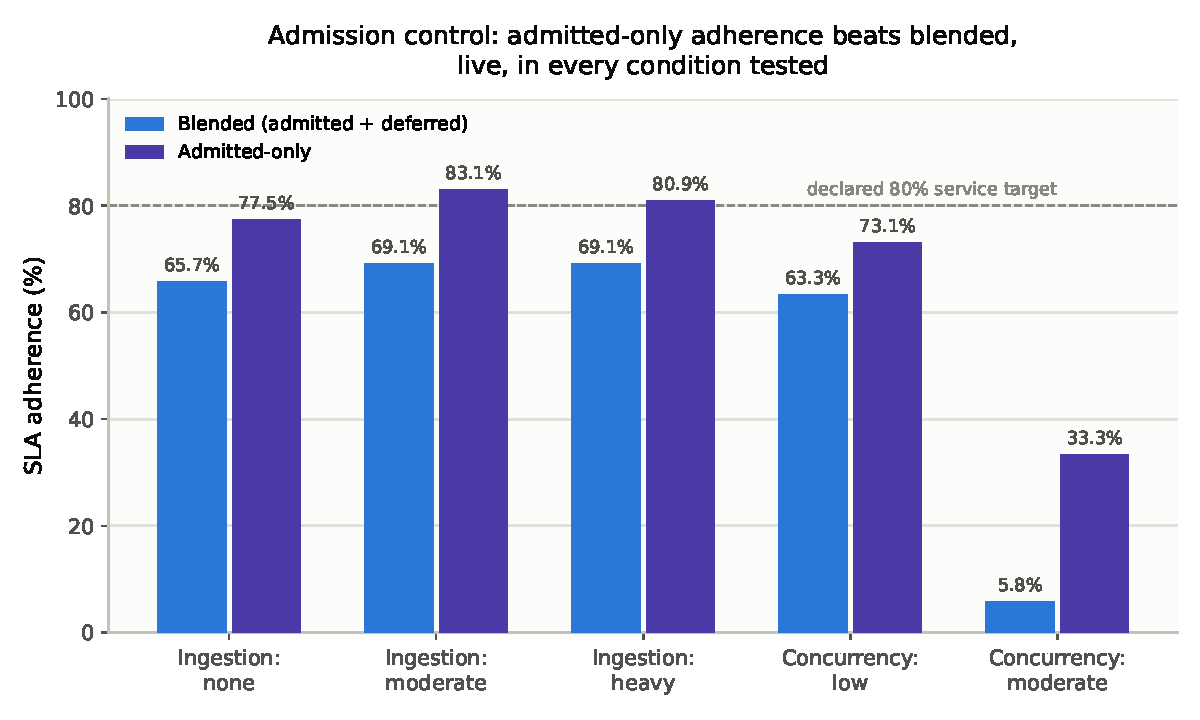
\includegraphics[width=\columnwidth]{figures/fig3_admission_control_live.pdf}
\caption{Blended (admitted + deferred) versus admitted-only SLA adherence, across every live condition tested.}
\label{fig:admission-live}
\end{figure}

Across all five live conditions tested -- three ingestion levels and two concurrency levels -- admitted queries met their deadlines more often than the blended average, which includes queries deliberately deferred (Fig.~\ref{fig:admission-live}). Deferred queries showed exactly 0\% adherence in every condition, confirming that the scoring is applied honestly: a deferred query is not excluded from accounting but scored as an ordinary miss once it eventually executes, last, after every admitted query.

The most notable result: under live moderate-concurrency contention, the admission controller deferred \textbf{82.5\%} of arriving queries after its predicted feasibility test classified further admission as unsafe. This is a live instance of the mechanism acting on predicted infeasibility, not a figure produced only in simulation. Whether every deferred query would in fact have missed its deadline if admitted is a separate question from whether the predicted test fired correctly; the live shortfall discussed below shows that this prediction is not perfectly calibrated under this same condition.

\begin{figure}[t]
\centering
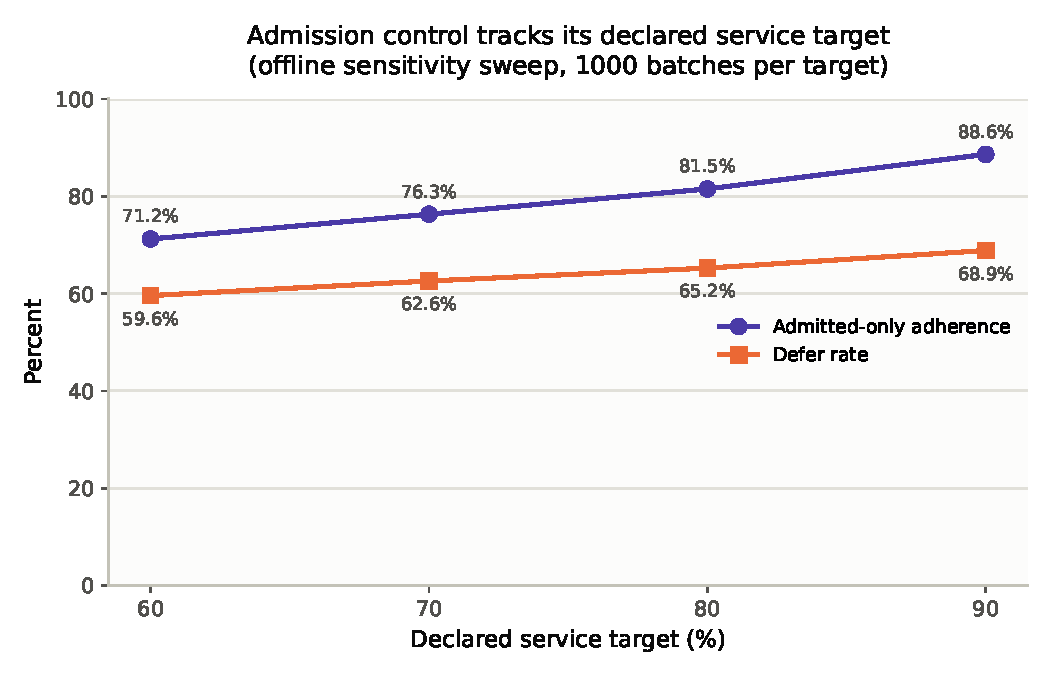
\includegraphics[width=\columnwidth]{figures/fig4_admission_sensitivity.pdf}
\caption{Admitted-only adherence and defer rate as the declared service target is varied (offline sensitivity sweep).}
\label{fig:admission-sensitivity}
\end{figure}

The declared service target (default 80\%) is a policy parameter rather than a value derived from data, and we tested its sensitivity (Fig.~\ref{fig:admission-sensitivity}): sweeping it from 60\% to 90\% moves admitted-only adherence from 71.2\% to 88.6\% monotonically and predictably, consistent with the target functioning as intended.

One result is reported without qualification: at live moderate concurrency specifically, admitted-only adherence (33.3\%) fell substantially short of the 80\% target, unlike every other tested condition, where admitted-only adherence met or approached target. We attribute this to a mismatch between the admission gate's feasibility predictions, which are built from discrete-round concurrency measurements, and the live concurrency test's continuous background load, which likely produces denser real contention than the calibration data assumed.

This attribution is not just a belief: we measured it directly. Table~\ref{tab:prediction-error} reports held-out prediction error for the Adaptive predictor (the same \texttt{predicted\_adaptive[(class, tier)]} value the DP-based schedulers and the admission gate use), scored against \texttt{concurrency\_contention\_heldout.csv}, a genuinely separate collection round. Median absolute percentage error (MAPE) at moderate concurrency is 30.6\% -- roughly four times higher than at low (8.0\%) or high (7.2\%) concurrency. Prediction error is not uniformly bad; it is specifically worse at the exact tier where the admission-control shortfall occurred, consistent with (though not full proof of) the discrete-round-versus-continuous-load explanation above.

\begin{table}[t]
\caption{Held-out prediction error, Adaptive predictor, pooled across query classes per concurrency tier (excludes two class/tier cells with no genuinely independent held-out sample; see Section~\ref{sec:limitations}).}
\label{tab:prediction-error}
\centering
\begin{tabular}{@{}lrrr@{}}
\toprule
\textbf{Tier} & \textbf{n} & \textbf{MAE (ms)} & \textbf{MAPE (\%)} \\
\midrule
Low & 8 & 23.0 & 8.0 \\
Moderate & 96 & 746.2 & 30.6 \\
High & 128 & 448.2 & 7.2 \\
\bottomrule
\end{tabular}
\end{table}

This discrepancy is not fully disentangled and is reported as an open gap between live-testing and calibration methodology, not as evidence against the admission-control mechanism itself: even with feasibility predictions measurably worse at this condition, the mechanism responded with aggressive deferral, which -- given that admitted-only adherence remained well below target even after deferral -- was the directionally appropriate response.

\subsection{Robustness Checks}
\label{sec:robustness}

Two values in this design are declared policy choices rather than measurements, and both are checked rather than assumed: the priority weights ($\{$priority~1:~3, priority~2:~2, priority~3:~1$\}$) and the admission-control service target (Section~\ref{sec:admission}). The priority weights are not a cosmetic reporting detail: they are the weight vector in the weighted-SLA objective that the DP-based schedulers (DP Oracle, Admission-Controlled DP) actually optimize when selecting an ordering (Section~\ref{sec:problem}); FIFO, Priority-First, EDF, and the Static/Adaptive Least-Slack heuristics never reference these weights, since their ordering rules use deadline and predicted slack directly. Because the weights are a live input to the DP objective rather than a cosmetic label, sweeping them constitutes a genuine test of the schedulers' actual decisions rather than of their reporting: across four weightings, including a uniform 1:1:1 weighting under which priority has no effect on scoring or on the DP schedulers' chosen ordering, the core finding is unchanged -- DP Oracle and Admission-Controlled DP lead every other scheduler at every weighting tested, and Admission-Controlled DP's protection of priority-1 queries tracks DP Oracle's closely regardless of the exact weights chosen. That this ranking survives variation in an input the DP objective genuinely uses is a stronger robustness result than would be obtained by sweeping a purely cosmetic parameter.

\section{Discussion}

Taken together, Sections~\ref{sec:ingestion} and~\ref{sec:results} support a specific practical recommendation: schedule intelligently while capacity exists, and detect -- rather than silently ignore -- the point at which it does not. Below saturation, concurrency-aware prediction materially changes scheduling decisions, and global DP-based scheduling provides additional opportunity to improve SLA adherence. Beyond a certain concurrency level, no ordering strategy helps, and the more defensible system response is admission control: informing some queries that they will execute later, rather than admitting all of them and allowing most to miss their deadlines.

This result also reframes what ``ingestion-aware'' scheduling should have meant for this project. It does not imply that ingestion contention is never relevant in any lakehouse deployment -- only that, at the scale and architecture evaluated here, it was not the bottleneck, and a scheduler built around the wrong bottleneck would not have improved outcomes. Testing this assumption explicitly, and revising the design once it failed, is itself a contribution of this work.

\section{Limitations and Threats to Validity}
\label{sec:limitations}

\textbf{Point predictions, not distributions.} Every scheduler in this paper predicts a single value (the median observed runtime for a given query class and concurrency level) rather than a range or probability distribution. A scheduler that reasoned explicitly about predictive uncertainty might behave differently, particularly near a deadline boundary. We did not build or evaluate such a scheduler; a future extension of this work should compare it directly against the point-prediction schedulers reported here. The held-out prediction-error check in Table~\ref{tab:prediction-error} is itself limited: the low-concurrency tier has a genuinely independent held-out sample for only one of three query classes ($n{=}8$), since the calibration sweep only cycles the \texttt{short} class at $C{=}1$; the other two classes at that tier fall back to resampling the calibration pool and are excluded from the aggregate.

\textbf{Live testing is sensitive to machine state, for reasons not fully diagnosed.} During live concurrency testing, uncontended query latency drifted well above the calibration baseline for reasons that could not be fully diagnosed; ingestion load, resource contention (CPU, memory, other processes), and network issues were each ruled out, but the root cause was not identified. Restarting the query engine and rerunning a warm-up routine restored baseline performance. We now check for this condition before every live session (Section~\ref{sec:setup}) and treat it as a methodological control, but the underlying sensitivity of single-node home-lab hardware to this kind of drift is itself a limitation on the session-to-session reproducibility of the live results.

\textbf{Concurrency is measured coarsely.} We use three concurrency levels (low, moderate, high), corresponding to approximately 1, 4--8, and 16 simultaneous queries. This granularity is sufficient to show that low concurrency performs well, moderate concurrency is already degraded, and high concurrency is saturated, but it is not sufficient to support a specific ``safe concurrency limit'' claim (e.g., that the system supports up to some fixed number of concurrent queries). A finer sweep would be required to support such a claim.

\textbf{Small live sample sizes.} Live results are drawn from dozens to a few hundred queries per condition, versus thousands in simulation. We treat the live results as confirmation that the offline ranking transfers to a real deployment, not as a precise estimate in their own right.

\textbf{Priority-aware admission control is out of scope.} The admission-control mechanism evaluated here is not priority-aware: it applies a single system-wide feasibility check rather than deferring lower-priority queries preferentially under overload. Extending the mechanism to defer by priority under overload is a natural next step not implemented here.

\textbf{Single hardware configuration.} All results are drawn from one specific single-node machine. It is not known how these findings would generalize to a true multi-node cluster, where the 19$\times$ concurrency slowdown measured here -- a direct consequence of running on a single node -- may not replicate.

\section{Related Work}

We review six areas relevant to this paper's claims and then position our contribution against them.

\textbf{SLA-aware scheduling.} Chi et al.~\cite{chi2013distribution} schedule against a predicted-cost \emph{distribution}, not a point estimate; a follow-up~\cite{chi2011icbs} makes this tractable online. Sabek et al.~\cite{sabek2022lsched} replace the scheduling rule with a learned RL policy. Each improves the scheduling \emph{rule}; we instead hold the rule fixed (least-slack or exact DP) and ask a narrower question -- what signal it should condition on.

\textbf{Admission control.} Mehta et al.~\cite{mehta2008biworkload} gate admission on memory in an enterprise warehouse batch manager; WiSeDB~\cite{marcus2016wisedb} learns admission, placement, and scheduling jointly; Kang, Son, and Stankovic~\cite{kang2004deadline} bound deadline miss ratio in real-time databases -- the same quantity we report (Section~\ref{sec:admission}). Our mechanism is deliberately simpler than any of these (one feasibility threshold, no learning, no per-resource accounting); its contribution is that it was evaluated live, including the one condition where it underperformed target.

\textbf{Concurrency-aware runtime prediction.} Duggan et al.~\cite{duggan2011performance} and Wu et al.~\cite{wu2013towards} model runtime degradation under concurrency; Wu et al.~\cite{wu2013predicting} show calibrated optimizer cost models predict well for admission and scheduling; Wu et al.~\cite{wu2014uncertainty} predict distributions rather than points, relevant to the limitation in Section~\ref{sec:limitations}. Most relevant is Wu et al.~\cite{wu2025iconqsched} (IconqSched): a bidirectional LSTM over query-plan features, far finer-grained than our three-tier signal -- a real limitation of this work -- feeding a greedy scheduler validated live on Postgres/Redshift. Two things distinguish our problem from~\cite{wu2025iconqsched} beyond granularity, however. First, IconqSched optimizes total/tail runtime with no per-query deadline or admission concept; by the authors' own words it ``does not reject or preempt queries, so [a queued query] will eventually be executed at some point,'' and SLA/SLO scheduling is named only as future work. Meeting a per-query deadline and deferring queries for which that is infeasible (Section~\ref{sec:admission}) is a different problem. Second, \cite{wu2025iconqsched} targets Postgres/Redshift, not a compute/storage-separated engine such as Trino. Our prediction step is a coarser version of what \cite{duggan2011performance,wu2013towards,wu2025iconqsched} already do with more sophistication, but our deadline and admission-control results address a question outside their scope.

\textbf{Trino resource management.} Sethi et al.~\cite{sethi2019presto} describe the Presto/Trino architecture this deployment instantiates. Trino's resource groups~\cite{trino2026resourcegroups} cap concurrency and memory per workload but do not reason about a query's predicted runtime against its deadline. Our mechanism could sit above resource groups rather than replace them; we do not evaluate that combination.

\textbf{Non-preemptive scheduling theory.} Liu and Layland~\cite{liu1973scheduling} show preemptive EDF achieves full utilization; Jeffay, Stanat, and Martel~\cite{jeffay1991nonpreemptive} give feasibility conditions for the non-preemptive case our schedulers operate under (Section~\ref{sec:problem}). That even the DP Oracle reaches 0\% adherence at high concurrency (Section~\ref{sec:results}) matches this classical result rather than being a new finding: once load exceeds capacity, no non-preemptive ordering can satisfy every deadline.

\textbf{Lakehouse contention.} Armbrust et al.~\cite{armbrust2021lakehouse} motivate the lakehouse architecture this deployment instantiates; Delta Lake~\cite{armbrust2020deltalake} is one such storage layer. Cheng et al.~\cite{cheng2025fair} study transaction-level fairness under multi-tenant contention, a related but distinct concern. A recent study~\cite{schiavo2026noisyneighbor} quantifies general-cloud noisy-neighbor degradation, consistent in direction with our 19$\times$ finding but not lakehouse-specific. We found no prior work measuring SLA-adherence under concurrent-query contention on a compute/storage-separated deployment; if that gap is real, our live single-node measurements (Sections~\ref{sec:results},~\ref{sec:limitations}) contribute toward it, for one hardware configuration.

\textbf{Positioning.} No individual component here is novel -- least-slack scheduling, deadline-miss-ratio admission control, DP as an objective-optimal benchmark, and EDF-style reasoning are each decades old. The closest prior work, Wu et al.~\cite{wu2025iconqsched}, already conditions prediction on concurrency with far finer granularity than our three-tier signal, and validates it live, so live validation alone does not distinguish us from it specifically (it does distinguish us from most other work reviewed, which is offline-only). What~\cite{wu2025iconqsched} does not do is per-query deadlines or admission control at all: every query it schedules is eventually run, and SLA/SLO scheduling is named only as unbuilt future work.

Given this, our claims are narrow: (1) an explicit, falsifiable test ruled out ingestion before adopting concurrency as the scheduling signal (Section~\ref{sec:ingestion}) -- a methodological point, not a new predictor; (2) live validation against real Trino of both the scheduler ranking and, specifically, the admission-control deferral behavior that~\cite{wu2025iconqsched} neither builds nor evaluates, including a live shortfall reported rather than omitted (Section~\ref{sec:admission}); (3) a deliberately simple, auditable admission gate, robustness-checked under a target sweep and a priority-weight sweep (Sections~\ref{sec:admission},~\ref{sec:robustness}). We do not claim a new algorithm or predictor, and our prediction signal is coarser than the state of the art~\cite{wu2025iconqsched}. We claim that a simple combination of established ideas, conditioned on an empirically validated signal and checked live rather than only in simulation, is a useful, honestly reported data point for SLA-aware scheduling on a comparable lakehouse deployment.

\section{Conclusion}

This work set out to test whether ingestion load is the dominant source of SLA risk in a lakehouse query engine and found, across four independent tests, that it is not. Query concurrency is the dominant factor: a single-node Trino deployment slows by a factor of 19 at sixteen concurrent queries relative to one, and this effect dominates scheduling decisions in a way ingestion did not. Reframing the scheduling problem around concurrency, we show that DP-based schedulers meaningfully outperform simple heuristics in aggregate, both in simulation and live against Trino, and that this ranking is stable under scoring against independently collected data. We further show that once concurrency exceeds a feasibility threshold, no scheduling policy can preserve SLA compliance, and that admission control -- recognizing this condition and deferring rather than over-promising -- is the more useful response: the admission-controlled scheduler's admitted-only adherence exceeded its blended adherence in every condition tested, live and simulated, and under live moderate-concurrency contention it deferred 82.5\% of incoming queries after its predicted feasibility test classified them as unsafe to admit.

We report this null effect of ingestion, at the scale and architecture tested here, as a rigorously tested finding in its own right -- not a universal claim that ingestion contention never matters -- and we state the limitations of this work explicitly: predictions are point estimates rather than distributions, concurrency is modeled at three coarse levels, and one live admission-control result fell short of what simulation predicted, for reasons not yet fully explained. We identify this last discrepancy as the most promising direction for follow-up work.

\section*{Data and Code Availability}

All results reported in this paper are derived from files in \texttt{results/week4/} and the accompanying analysis scripts in \texttt{scripts/}, within the project repository. Key result files include \texttt{results/week4/simulation\_report.md}, \texttt{results/week4/live\_concurrency\_validation\_report.md}, and \texttt{results/week4/admission\_control\_live\_reconciliation.md}; the full scheduler design rationale is documented in \texttt{research-plan/week4\_scheduler\_design.md}.

\bibliographystyle{IEEEtran}
\bibliography{refs}

\end{document}
